% Options for packages loaded elsewhere
\PassOptionsToPackage{unicode}{hyperref}
\PassOptionsToPackage{hyphens}{url}
\PassOptionsToPackage{dvipsnames,svgnames,x11names}{xcolor}
%
\documentclass[
  9pt,
  twocolumn,
  twoside]{pnas-new}

\usepackage{amsmath,amssymb}
\usepackage{iftex}
\ifPDFTeX
  \usepackage[T1]{fontenc}
  \usepackage[utf8]{inputenc}
  \usepackage{textcomp} % provide euro and other symbols
\else % if luatex or xetex
  \usepackage{unicode-math}
  \defaultfontfeatures{Scale=MatchLowercase}
  \defaultfontfeatures[\rmfamily]{Ligatures=TeX,Scale=1}
\fi
\usepackage{lmodern}
\ifPDFTeX\else  
    % xetex/luatex font selection
\fi
% Use upquote if available, for straight quotes in verbatim environments
\IfFileExists{upquote.sty}{\usepackage{upquote}}{}
\IfFileExists{microtype.sty}{% use microtype if available
  \usepackage[]{microtype}
  \UseMicrotypeSet[protrusion]{basicmath} % disable protrusion for tt fonts
}{}
\makeatletter
\@ifundefined{KOMAClassName}{% if non-KOMA class
  \IfFileExists{parskip.sty}{%
    \usepackage{parskip}
  }{% else
    \setlength{\parindent}{0pt}
    \setlength{\parskip}{6pt plus 2pt minus 1pt}}
}{% if KOMA class
  \KOMAoptions{parskip=half}}
\makeatother
\usepackage{xcolor}
\setlength{\emergencystretch}{3em} % prevent overfull lines
\setcounter{secnumdepth}{-\maxdimen} % remove section numbering
% Make \paragraph and \subparagraph free-standing
\ifx\paragraph\undefined\else
  \let\oldparagraph\paragraph
  \renewcommand{\paragraph}[1]{\oldparagraph{#1}\mbox{}}
\fi
\ifx\subparagraph\undefined\else
  \let\oldsubparagraph\subparagraph
  \renewcommand{\subparagraph}[1]{\oldsubparagraph{#1}\mbox{}}
\fi


\providecommand{\tightlist}{%
  \setlength{\itemsep}{0pt}\setlength{\parskip}{0pt}}\usepackage{longtable,booktabs,array}
\usepackage{calc} % for calculating minipage widths
% Correct order of tables after \paragraph or \subparagraph
\usepackage{etoolbox}
\makeatletter
\patchcmd\longtable{\par}{\if@noskipsec\mbox{}\fi\par}{}{}
\makeatother
% Allow footnotes in longtable head/foot
\IfFileExists{footnotehyper.sty}{\usepackage{footnotehyper}}{\usepackage{footnote}}
\makesavenoteenv{longtable}
\usepackage{graphicx}
\makeatletter
\def\maxwidth{\ifdim\Gin@nat@width>\linewidth\linewidth\else\Gin@nat@width\fi}
\def\maxheight{\ifdim\Gin@nat@height>\textheight\textheight\else\Gin@nat@height\fi}
\makeatother
% Scale images if necessary, so that they will not overflow the page
% margins by default, and it is still possible to overwrite the defaults
% using explicit options in \includegraphics[width, height, ...]{}
\setkeys{Gin}{width=\maxwidth,height=\maxheight,keepaspectratio}
% Set default figure placement to htbp
\makeatletter
\def\fps@figure{htbp}
\makeatother
% definitions for citeproc citations
\NewDocumentCommand\citeproctext{}{}
\NewDocumentCommand\citeproc{mm}{%
  \begingroup\def\citeproctext{#2}\cite{#1}\endgroup}
\makeatletter
 % allow citations to break across lines
 \let\@cite@ofmt\@firstofone
 % avoid brackets around text for \cite:
 \def\@biblabel#1{}
 \def\@cite#1#2{{#1\if@tempswa , #2\fi}}
\makeatother
\newlength{\cslhangindent}
\setlength{\cslhangindent}{1.5em}
\newlength{\csllabelwidth}
\setlength{\csllabelwidth}{3em}
\newenvironment{CSLReferences}[2] % #1 hanging-indent, #2 entry-spacing
 {\begin{list}{}{%
  \setlength{\itemindent}{0pt}
  \setlength{\leftmargin}{0pt}
  \setlength{\parsep}{0pt}
  % turn on hanging indent if param 1 is 1
  \ifodd #1
   \setlength{\leftmargin}{\cslhangindent}
   \setlength{\itemindent}{-1\cslhangindent}
  \fi
  % set entry spacing
  \setlength{\itemsep}{#2\baselineskip}}}
 {\end{list}}
\usepackage{calc}
\newcommand{\CSLBlock}[1]{\hfill\break\parbox[t]{\linewidth}{\strut\ignorespaces#1\strut}}
\newcommand{\CSLLeftMargin}[1]{\parbox[t]{\csllabelwidth}{\strut#1\strut}}
\newcommand{\CSLRightInline}[1]{\parbox[t]{\linewidth - \csllabelwidth}{\strut#1\strut}}
\newcommand{\CSLIndent}[1]{\hspace{\cslhangindent}#1}

% TODO: Add custom LaTeX header directives here
\makeatletter
\@ifpackageloaded{caption}{}{\usepackage{caption}}
\AtBeginDocument{%
\ifdefined\contentsname
  \renewcommand*\contentsname{Table of contents}
\else
  \newcommand\contentsname{Table of contents}
\fi
\ifdefined\listfigurename
  \renewcommand*\listfigurename{List of Figures}
\else
  \newcommand\listfigurename{List of Figures}
\fi
\ifdefined\listtablename
  \renewcommand*\listtablename{List of Tables}
\else
  \newcommand\listtablename{List of Tables}
\fi
\ifdefined\figurename
  \renewcommand*\figurename{Figure}
\else
  \newcommand\figurename{Figure}
\fi
\ifdefined\tablename
  \renewcommand*\tablename{Table}
\else
  \newcommand\tablename{Table}
\fi
}
\@ifpackageloaded{float}{}{\usepackage{float}}
\floatstyle{ruled}
\@ifundefined{c@chapter}{\newfloat{codelisting}{h}{lop}}{\newfloat{codelisting}{h}{lop}[chapter]}
\floatname{codelisting}{Listing}
\newcommand*\listoflistings{\listof{codelisting}{List of Listings}}
\makeatother
\makeatletter
\makeatother
\makeatletter
\@ifpackageloaded{caption}{}{\usepackage{caption}}
\@ifpackageloaded{subcaption}{}{\usepackage{subcaption}}
\makeatother
\ifLuaTeX
  \usepackage{selnolig}  % disable illegal ligatures
\fi
\usepackage{bookmark}

\IfFileExists{xurl.sty}{\usepackage{xurl}}{} % add URL line breaks if available
\urlstyle{same} % disable monospaced font for URLs
\hypersetup{
  pdftitle={Switchgrass Phenology and Genotype-by-Environment Mapping},
  pdfauthor={Alice H. MacQueen; Li Zhang; Samuel A. Smith; Jason Bonnette; Arvid R. Boe; Phillip A. Fay; Felix B. Fritschi; David B. Lowry; Robert B. Mitchell; Francis M. Rouquette Jr; Yanqi Wu; Arbel Harpak; Thomas E. Juenger},
  pdfkeywords={allele-by-environment effect variation, antagonistic
pleiotropy, photoperiod, cumulative rainfall, genetic variation},
  colorlinks=true,
  linkcolor={blue},
  filecolor={Maroon},
  citecolor={Blue},
  urlcolor={Blue},
  pdfcreator={LaTeX via pandoc}}

\templatetype{pnasresearcharticle}

\title{Switchgrass Phenology and Genotype-by-Environment Mapping}

\newcommand{\equalcont}{1}

\newcommand{\correspond}{2}

\author[a%
,\equalcont%
,\correspond%
]{Alice H. MacQueen}
\author[a%
,\equalcont%
%
]{Li Zhang}
\author[a%
,\equalcont%
%
]{Samuel A. Smith}
\author[a%
%
%
]{Jason Bonnette}
\author[b%
%
%
]{Arvid R. Boe}
\author[c%
%
%
]{Phillip A. Fay}
\author[d%
%
%
]{Felix B. Fritschi}
\author[e%
%
%
]{David B. Lowry}
\author[f%
%
%
]{Robert B. Mitchell}
\author[g%
%
%
]{Francis M. Rouquette Jr}
\author[h%
%
%
]{Yanqi Wu}
\author[a%
%
%
]{Arbel Harpak}
\author[a%
%
,\correspond%
]{Thomas E. Juenger}

\affil[a]{University of Texas at Austin, Department of Integrative
Biology, Austin, 78712}
\affil[b]{South Dakota State University, Department of
Agronomy, Brookings, 57006}
\affil[c]{USDA-ARS, Grassland, Soil and Water Research
Laboratory, Temple, 76502}
\affil[d]{University of Missouri, Division of Plant
Sciences, Columbia, 65211}
\affil[e]{Michigan State University, Department of Plant Biology, East
Lansing, 48824}
\affil[f]{USDA-ARS, Wheat, Sorghum, and Forage Research
Unit, Lincoln, 68583}
\affil[g]{Texas A\&M University, Texas A\&M AgriLife Research and
Extension Center, Overton, 75684}
\affil[h]{Oklahoma State University, Department of Plant and Soil
Sciences, Stillwater, 74078}

\leadauthor{MacQueen}

\significancestatement{The timing of plant seasonal development
(phenology) has major impacts on fitness because of the steep price of
plant-environment mismatches. We infer the mixture of ways genetic
effects on phenological traits depend on plant environment, particularly
how effects covary with weather prior to the phenological event
(GxWeather). Most effects do not have GxWeather, but a minority do.
GxWeather is population-specific. The majority of effects on the start
of vegetative growth in the Gulf population have GxWeather: these
effects differ in sign across environments and covary with a photoperiod
cue 14 days prior. A minority of effects on flowering date in the Gulf
and Midwest populations had GxWeather, covarying with a cumulative
rainfall and a photoperiod cue, respectively.}

\authorcontributions{T.E.J. designed research. D.B.L. contributed plant
material and resources. J.B., D.B.L., and T.E.J. designed and executed
field experiments. A.R.B., P.A.F., F.B.F., D.B.L., R.B.M., F.M.R., Y.W.,
and T.E.J. hosted field experiments. A.H.M., L.Z., and S.A.S. conducted
statistical and computational analyses. The manuscript was written by
A.H.M. with contributions from all authors.}

\authordeclaration{The authors declare no conflicts of interest.}

\equalauthors{\textsuperscript{\equalcont} A.H.M. contributed equally to
this work with L.Z. and S.A.S.}

\correspondingauthor{\textsuperscript{\correspond}To whom correspondence should be addressed. E-mail: alicem@uchicago.edu}
\correspondingauthor{\textsuperscript{\correspond}To whom correspondence should be addressed. E-mail: tjuenger@utexas.edu}

\keywords{allele-by-environment effect variation | antagonistic
pleiotropy | photoperiod | cumulative rainfall | genetic variation}

\begin{document}
\maketitle

\begin{abstract}
The timing of vegetative growth and flowering in plants (``phenological
timings'') depend on both genetic variation and environmental cues;
thus, phenological traits can have important genotype-by-environment
(GxE) interactions. In particular, understanding the mixture and
prevalence of genotype-by-weather (GxWeather) interactions primed by
weather prior to the phenological event should aid prediction and
manipulation of phenological timings. Here, we map genotype-by-weather
effects on phenological timings in two highly divergent switchgrass
(\emph{Panicum virgatum}) populations using repeated plantings of these
populations at sites spanning the central United States. We distinguish
GxWeather patterns covarying with interpretable weather-based cues from
agnostic, site-based patterns. Most GxWeather effects belong to the
latter category and do not covary with weather-based cues. However, 65\%
of Gulf population effects on the start of vegetative growth covary with
daylength 14 days prior to green-up date. 33\% of Gulf population
effects on flowering date covary with cumulative rainfall in the seven
days prior to flowering, while 22\% of Midwest population effects on
flowering date covaried with day length change two days prior to
flowering. An independent pseudo-F2 cross of Gulf and Midwest
individuals mapped 23 additive QTLs for flowering at the same common
gardens, all with significant mash associations and eleven with
enrichment of highly significant mash associations. We demonstrate that
we can identify QTL with GxWeather and assign them to specific
weather-based cues or other patterns. Breeding for particular alleles at
these loci could change flowering responsiveness to photoperiod cues in
switchgrass. More broadly, this approach could be used to identify
genetic marker-environment interactions in any species with related
populations phenotyped in multiple environments.
\end{abstract}

\dates{This manuscript was compiled on \today}
\doi{\url{www.pnas.org/cgi/doi/10.1073/pnas.XXXXXXXXXX}}

\thispagestyle{firststyle}
\ifthenelse{\boolean{shortarticle}}{\ifthenelse{\boolean{singlecolumn}}{\abscontentformatted}{\abscontent}}{}
\firstpage[10]{2}

The timing of plant vegetative and reproductive development are major
components of plant fitness affected by multiple external environmental
cues (e.g.~degree of winter chilling, day length, temperature, and water
availability) that signal existing or upcoming growing conditions
(1--3). Genetic responses to environmental cues determine the speed,
timing, and energy apportioned to vegetative and reproductive growth and
shape both the individual's lifespan and its lifetime production of
viable seed. Day length (or photoperiod) is one of the most predictable
environmental cues, and genetic sensitivity to photoperiod protects
plants from potentially fatal consequences of phenological responses to
temperature cues at the ``wrong'' time of year. However, the usefulness
of specific environmental cues depends on both features of the
environment and the species' adaptive strategies (4). Species with wide
natural distributions can have multiple distinct environmentally-cued
phenological responses: for example, populations of sunflower
(Helianthus annuus) exhibit day-neutral, facultative short day, and
facultative long-day flowering responses, which vary with their
environments (5, 6). Distinct genetic responses in different
environments are known as genotype by environment interactions, or GxE.

Flowering time, in particular, is a common subject of GxE research
(5--11), a key output of selection driving adaptation to local
environments (2, 12, 13), and a selection target for crop improvement to
adapt crops to local or future environments (14). Changing flowering
responsiveness to photoperiod cues has allowed geographic range
expansion and increased yields in a number of cereal species (15--19)
and other crops (20, 21). Recent statistical advances in studying
phenological GxE have involved determining critical environmental
indices before the phenological event occurs, such as photothermal time
within a critical growth window (10). However, most studies of flowering
GxE focus on finding a single, best fitting form of genotype-environment
covariance, despite the key expectation that different genetic
subpopulations, and even different genomic regions, have likely evolved
distinct patterns of GxE. Additionally, despite theoretical predictions
that local adaptation should involve antagonistic pleiotropy, or
sign-changing GxE, at the level of individual loci (22--25), previous
work has found limited evidence of antagonistic pleiotropy (12, 26), but
has been limited by a known statistical bias that reduced detection of
genetic effects that differ in sign (26--28). Thus, despite substantial
interest in the frequencies of various forms of GxE, the prevalence of
antagonistic pleiotropy relative to other forms of GxE remains unknown.

Switchgrass (\emph{Panicum virgatum}) is considered a short-day plant
with reproductive development strongly linked to day of the year (29).
However, as part of its wide environmental adaptation across the eastern
half of North America, its photoperiodicity has been predicted to differ
by plant latitude of origin (30, 31). We previously found divergent
Midwest and Gulf genetic subpopulations of switchgrass which segregate
for distinct sets of environmental adaptations, based on the analysis of
two measures of fitness (i.e.,biomass and survival) among 732 genotypes
(32). The Midwest genetic subpopulation is primarily composed of
individuals from the well-studied upland switchgrass ecotype (33, 34),
while the Gulf subpopulation has individuals from the lowland ecotype
and the phenotypically intermediate coastal ecotype (32).

Here, we test how the Midwest and Gulf subpopulations differ in their
phenological adaptations across environments, and hence their
phenological GxE. We phenotype a diversity panel of hundreds of
switchgrass genotypes from the Midwest and Gulf subpopulations for the
timing of vegetative development (``green-up'') and reproductive
development (flowering) at eight common garden locations spanning 17
degrees of latitude. These gardens cover the majority of the latitudinal
and climatic range of switchgrass and capture the most comprehensive
picture to date of the environmental variation this species encounters.
After single-site estimation of SNP effects for these phenotypes, we use
multivariate adaptive shrinkage (mash) to jointly estimate SNP effects
in each subpopulation and phenotype at all eight sites (35). Mash allows
us to identify and specify multiple ways genetic effects linked to SNPs
may covary with the environment, and does not have a statistical bias in
detecting SNP effects with the same or opposite signs (36). To confirm
our genetic mapping of GxE, we compare to mapping results from an
outbred pseudo-F2 cross grown at the same sites. Taken together, our
results allow us to describe the environmental cues and genetic
variation affecting phenology in two divergent natural populations of
switchgrass.

\section{Results}\label{results}

In our diversity panel of tetraploid switchgrass (32), genotypes from
the Gulf and Midwest genetic subpopulations had distinct phenological
timings and distinct patterns of phenological correlations across our
eight common garden sites (Figure~\ref{fig-map}). At the three Texas
common gardens (hereafter `Texas' gardens), located within the natural
range of the Gulf subpopulation, Gulf green-up occurred before
Midwestern green-up, and Gulf flowering occurred after Midwestern
flowering (Figure~\ref{fig-map} A). At the four northernmost common
gardens (hereafter `North' gardens), located within the natural range of
the Midwest subpopulation, both Gulf green-up and flowering occurred
after Midwest green-up and flowering. At the Oklahoma common garden,
located near the natural range limits of both the Gulf and the Midwest
subpopulations, Gulf and Midwest green-up occurred over the same time
period. These patterns led to strong negative phenotypic correlations
for green-up between the North and Texas gardens, particularly in the
Gulf and Both subpopulations, and contributed to positive phenotypic
correlations for flowering time of larger magnitude at more northern
gardens (Figure~\ref{fig-map} B).

Narrow-sense heritabilities (h\textsuperscript{2}) indicated that
rank-changing GxE for these phenotypes was present across the common
gardens (Fig 1C). h\textsuperscript{2} were typically high at individual
gardens: 59\% on average for green-up date, and 87\% for flowering date.
However, h2 were variable across gardens, and green-up dates were
uncorrelated (r2 \textless{} 0.2) or negatively correlated between pairs
of gardens (Fig. 1B). These negative and small correlations undoubtedly
contributed to the low h2 values for green-up and flowering date when
estimated jointly at all eight gardens: h2 was 0.8\% for green-up and
23.2\% for flowering date.

\subsubsection{Mapping major patterns of genotype-by-environment effects
on green-up and
flowering}\label{mapping-major-patterns-of-genotype-by-environment-effects-on-green-up-and-flowering}

We next explored how genetic variation in phenology covaried with
environmental cues by using mash to jointly discover trait-associated
SNPs across all common gardens for the Midwest, Gulf, and `Both'
subpopulations (Fig 1D, SI Appendix, Datasets 1-6). We first estimated
SNP effects using GWAS on site-specific BLUPs for each phenotype. We
then used mash on two subsets of these SNP effects, first to determine
the covariance structures that significantly improved the mash model log
likelihood when included, then to re-estimate the set of SNP effects
with the largest effect estimates in univariate GWAS (hereafter
``strong'' effects) using the set of significant covariance matrices.

Three types of covariance matrices were tested for inclusion:
``canonical'' covariance matrices, with simple patterns of effects;
``data-driven'' matrices derived from common patterns of SNP effects in
the data, and ``hypothesis-based'' covariance matrices that captured the
covariance of weather-based phenological cues for cloned genotypes grown
at multiple common gardens (Table 1, SI Appendix, Section S2). Mash
first assigns mixture proportions for each SNP onto each provided
covariance matrix using maximum likelihood. Then, in a second step, each
SNP's effect estimate undergoes shrinkage such that it is more aligned
with the covariance structure inferred in the first step. The
hypothesis-based covariance matrices are an important advantage mash
offers for studying patterns of GxE: they allow hypothesis testing of
specific environmental drivers for each SNP effect, and loadings on
these matrices provide information on genome-wide patterns of
SNP-environment interaction. Say that a SNP in FLC controls flowering in
a temperature-dependent manner. In that case, that SNP effect could have
a high mixture proportion, or mass, on a covariance matrix created using
a temperature-based environmental cue, such as average temperature on
the day prior to flowering. In our data, we would infer that the effect
of that SNP on flowering was caused by a response to that or a
correlated environmental cue.

The phenotypic correlations for green up date had moderate negative
correlations between the Texas and North gardens, particularly in the
Gulf and in Both subpopulations (Fig 1B). If these phenotypic
correlations have a genetic component, then they might be controlled by
SNP effects that differed in sign across these regions, SNP effects that
are large in one garden or region and non-significant in others, or a
combination of these patterns. Five hypothesis-based covariance matrices
were selected by the greedy mash algorithm, one to two per
subpopulation. Of these five, three had mass on them in mash models of
the strong effects (Fig 2A, 2B). Two of these three matrices had
negative covariances between sites between Texas and North gardens (Fig
2A), while one had all positive or near-zero covariances. SNP-associated
phenotypic effects covaried with different weather-based cues in the
Gulf \& in Both subpopulations (Fig 2B). In total, 65\% of the posterior
weight of strong SNP effects in the mash model of Gulf green-up fell on
a covariance matrix of daylength 14 days prior to the date of green-up.
The covariance matrix for this weather cue was very similar to the
pattern of phenotypic correlation for green-up in the Gulf subpopulation
(Fig 1B; Fig 2A). Mash models of Midwest and Both subpopulation green-up
did not include this covariance matrix; the Midwest had no weight on any
hypothesis-based matrix, while Both subpopulations had non-zero weights
on two additional hypothesis-based matrices, average temperature one day
prior to green-up, and the day length change in seconds in the day prior
to green-up (Fig 2B). The average temperature covariance matrix had
negative covariances between Texas and North gardens, though not as
strong as the negative phenotypic correlations seen in Both
subpopulations (Fig 1B; Fig 2A). Only the Gulf subpopulation and Both
subpopulations had mass on any hypothesis-based covariance matrices (Fig
2C).

For flowering date, distinct weather-based cues captured SNP-associated
effect patterns in the Gulf and Midwest subpopulations. 33\% of SNP
effects on flowering in the Gulf subpopulation covaried with cumulative
rainfall in the seven days prior to flowering (Fig 2D). 22.6\% of SNP
effects on flowering in the Midwest subpopulation contrived with day
length change in the two days prior to flowering (Fig 2D), which had
negative covariances between Texas and North gardens. Neither covariance
matrix was selected for in Both subpopulations, and no hypothesis-based
covariance matrices had mass in Both subpopulations (Fig 2E). In five of
the six mash models of strong effects, the hypothesis-based covariance
matrices captured a minority of the posterior weights of the strong
effects (Figure 2C,E); the majority of this mass was on various
canonical covariance matrices. These matrices included simple
heterozygosity, with intermediate, positive covariances between all
gardens, and garden-specific effects present only at one garden.

We next characterized the pairwise patterns of effects where we were
confident in the sign of the effect at both gardens. We used the local
false sign rate (lfsr), an analogue of the lfdr that establishes
confidence in the effect sign, not the effect's difference from zero, to
determine significance. We required significance (p \textless{} 0.05) in
both gardens to include effects. This means that our tests for
antagonistic pleiotropy, or a sign change between conditions, carry an
equal statistical burden to those for effects with the same sign. We
also summarized the pairwise patterns of effect sign and magnitude
within and between the Texas and North regions (Table 2).

For greenup date for the Gulf subpopulation, hundreds to thousands of
pairwise effects exhibited antagonistic pleiotropy, or a difference in
effect sign, between pairs of Texas and North gardens (Fig. 3A). 78.7\%
of pairwise comparisons between North and Texas gardens had a difference
in sign, while only 28.6\% and 0.2\% of North-North or Texas-Texas
comparisons had a difference in sign, respectively (Table 2). The
majority of pairwise effects for greenup for the Midwest
(\textgreater55\%) and Both (\textgreater85\%) subpopulations were the
same sign, and effects frequently differed in magnitude between the MO
and OK garden and other gardens (Table 2; Fig 3A).

For flowering date for the Gulf subpopulation, less than 2\% of pairwise
effects exhibited antagonistic pleiotropy, or a difference in effect
sign, within or between regions (Table 2). More effects differed in
magnitude between the Texas and North regions than within these regions
(42.7\% vs \textless20\%; Figure 3B). The Midwest population had
relatively few significant effects for flowering, but a large proportion
of these differed in sign between Texas and North regions (42.7\%) or
within the North region (65.4\%). Finally, in Both subpopulations, less
than 20\% of pairwise effects differed in sign (Table 2). Most
differences in sign were between TX1, the southernmost garden, and all
other gardens (Fig 3B). Similarly, more effects that differed in
magnitude included gardens in the Texas region (52.3-55.9\%), and most
effect pairs in the North region were not distinguishable (91.5\%).

\subsubsection{Confirmation of genotype-by-environment effects using an
independent mapping
population}\label{confirmation-of-genotype-by-environment-effects-using-an-independent-mapping-population}

We sought additional experimental support for our mash intervals using
an independent pseudo-F2 mapping population created from Gulf \& Midwest
individuals and grown at the same sites (Fig. 4A,B). We conducted
quantitative trait loci (QTL) mapping of flowering as functions of four
environmental cues that we also used as covariance matrices in mash, and
identified eight QTL for flowering date, six QTL for flowering GDD, ten
QTL for flowering day length, and eight QTL flowering day length change,
all of which showed QTL by environment interactions (SI Appendix, Fig.
S3). All QTL for flowering overlapped one or more homologs from rice or
A. thaliana with functionally validated roles in flowering (SI Appendix,
Dataset 7). All flowering QTL intervals contained at least one SNP
significant in at least one mash run at a log10-transformed Bayes Factor
\textgreater{} 2, or in the 1\% tail of significance, whichever was
stricter (SI Appendix, Dataset 8). We also looked for enrichments of
mash SNPs in the 1\% tail of significance (the `mash 1\% tail') within
each QTL interval. At the 5\% level, five QTL had enrichments of SNPs in
the mash 1\% tail. Overall, there were eleven significant enrichments (p
\textless{} 0.05, hypergeometric test) of SNPs in the mash 1\% tail in
the QTL intervals. Our QTL intervals had more enrichments of SNPs in the
mash 1\% tail than were found for all but eleven of these sets of random
genomic intervals (Fig. 4C, p = 0.011). Thus, we were able to
experimentally support our mash intervals with a QTL mapping experiment
using a separate mapping population.

\section{Discussion}\label{discussion}

As the climate and the natural environment change, it is increasingly
critical to understand how patterns of gene-environment and
plant-environment interactions will change in response. To do this, we
must understand the current patterns of trait covariation across
environments, the genetic underpinnings of these patterns, and the cases
where this covariation can be altered. Here, we demonstrate that we can
associate multiple patterns of GxE with specific genomic regions using a
switchgrass diversity panel grown at eight common gardens, and also that
we can assign specific SNP-associated patterns of GxE to both
weather-based cues and to other, data-driven patterns. We use this
approach to study GxE in both green-up and flowering phenological data
in the deeply genetically diverged Gulf and Midwest populations of
switchgrass.

Our analysis of green-up in the Gulf and in Both subpopulations revealed
substantial antagonistic pleiotropy in effects between the Texas and
North gardens (Figure 3A). This result supports theoretical models that
local adaptation should involve antagonistic pleiotropy at the level of
individual loci (22--25), and is the first experimental work using QTL
mapping and GWAS across common gardens to find antagonistic pleiotropy
to be common in small genomic regions (12, 36, 37).

Our analysis of flowering showed that the Gulf and Midwest
subpopulations have two distinct photoperiod-related flowering
responses: the Midwest subpopulation is day neutral, and flowering is
cued primarily by a cumulative GDD threshold; in contrast, the Gulf
subpopulation is photoperiod sensitive, and flowering is cued by the
transition to shortening days. This result was supported by observations
that expressing flowering date as a function of the day length at
flowering increased its heritability in the Gulf subpopulation, while
expressing flowering date as a function of cumulative GDD between
green-up and flowering increased the heritability of flowering in the
Midwest subpopulation (Fig. 1D). The genomic regions affecting flowering
found in mash were also supported by QTL from an independent mapping
population (Fig. 4C).

Identifying the environmental cues that are predictive of, or even
correlated with, plant phenotypic responses remains a major challenge to
studies interrogating gene action across many natural environments.
Clearly, the photoperiod and cumulative GDD cues we identify here are
functions of the genotypes measured, are not predictive, and capture
only a minority of SNP effects on flowering. We know still less about
the overwintering parameters that affect green-up, which is reflected in
our lower ability to assign SNP effects on green-up to weather-based
cues. More generally, it is difficult to predict the time scales over
which individuals may integrate environmental cues, particularly in
perennial species which may integrate these cues over longer time
scales. Mash offers an opportunity to specify multiple environmental
cues and compete them to explain patterns of SNP effects, allowing us to
detect how important these cues are genome-wide, and how strongly each
cue influences each SNP. This is a key development to further improve
our understanding of genetic variation in GxE.

\section{Figures and Tables}\label{figures-and-tables}

\begin{table}[t!]
\centering
\caption{Weather variables and time frames around the green up and flowering date used to construct the hypothesis-based covariance matrices. The correlations between values of these weather variables for genetically identical plants grown in different gardens were used to fill off-diagonal cells of the covariance matrices. Narrow-sense heritabilities for these values at each garden were used for the diagonal cells.}
\begin{tabular}{lrr}
Weather variable & Time Frame & Covariance Matrices tested \\
\midrule
1. cumulative GDD at 12C in the time frame & (1-7), 14, 21, 28 days prior to green up date & 60 \\
2. cumulative rainfall in the time frame & (1-7), 14, 21, 28 days prior to green up date & 60  \\
3. day length (hours) on a specific day indicated by the time frame & (1-7) and 14 days prior to green up date & 48 \\
4. day length change (seconds) on a specific day indicated by the time frame & (1-7) and 14 days prior to green up date & 48 \\
5. average temperature in the time frame & (1-7), 14, 21, 28 days prior to green up date & 60 \\
\bottomrule
\end{tabular}

\end{table}

\begin{figure}

\centering{

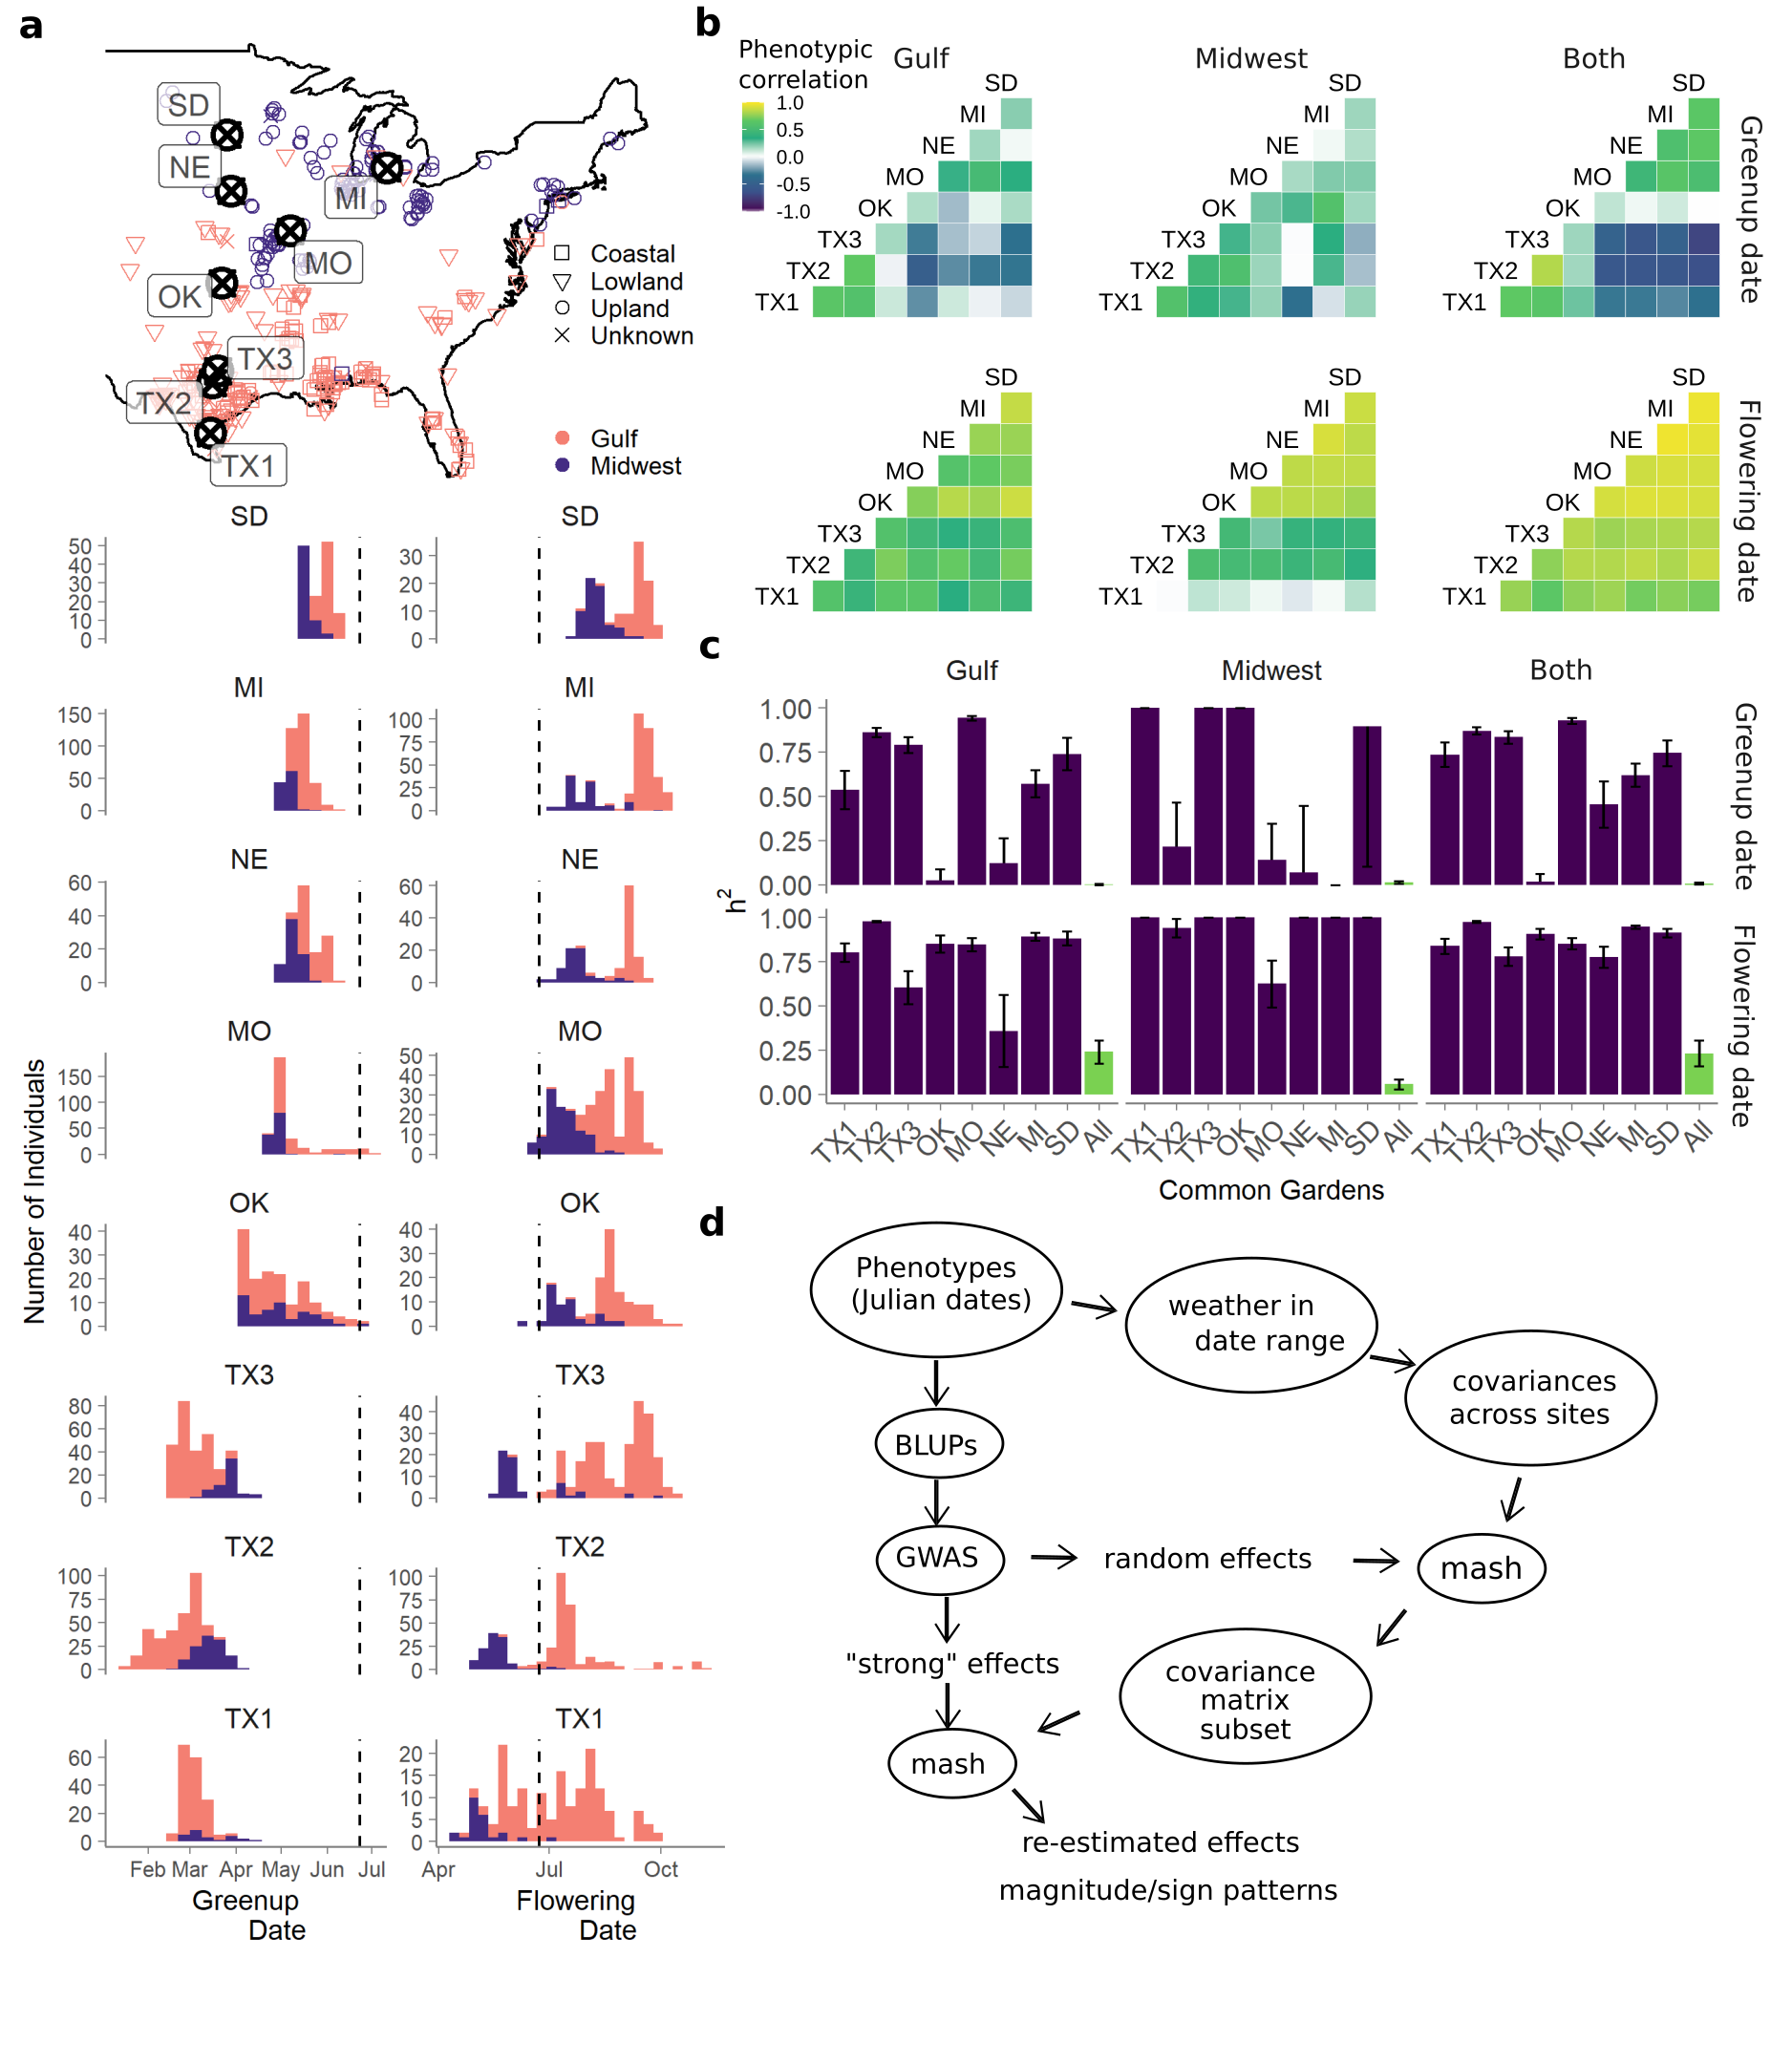
\includegraphics{images/Fig1_200dpi.png}

}

\caption{\label{fig-map}Figure 1. Characterization of green-up and
flowering dates from the switchgrass diversity panel. (a) Map and trait
histograms of green-up and flowering dates across two genetically
distinct switchgrass subpopulations and eight common gardens. Purple
represents individuals from the Midwest genetic subpopulation, and pink
individuals from the Gulf subpopulation. Vertical dashed lines indicate
the summer solstice. Common gardens are arranged in latitudinal order.
(b) Phenotypic correlations between clonal replicates planted at eight
common gardens, within and between two genetic subpopulations. (c)
Narrow sense heritability of green-up and flowering within single common
gardens (purple) and across all eight common gardens (green), within and
between two genetic subpopulations. (d) Flow diagram of the methods
applied to the green-up and flowering dates to jointly estimate SNP
effects across all sites. Mash was fit to SNP effect data and used to
find covariance matrices that improved the mash model likelihood using a
large set of randomly selected, relatively unlinked SNP effects; this
model was applied to a ``strong'' set of SNP effects with large effect
sizes in the univariate GWAS.}

\end{figure}%

\begin{figure}

\centering{

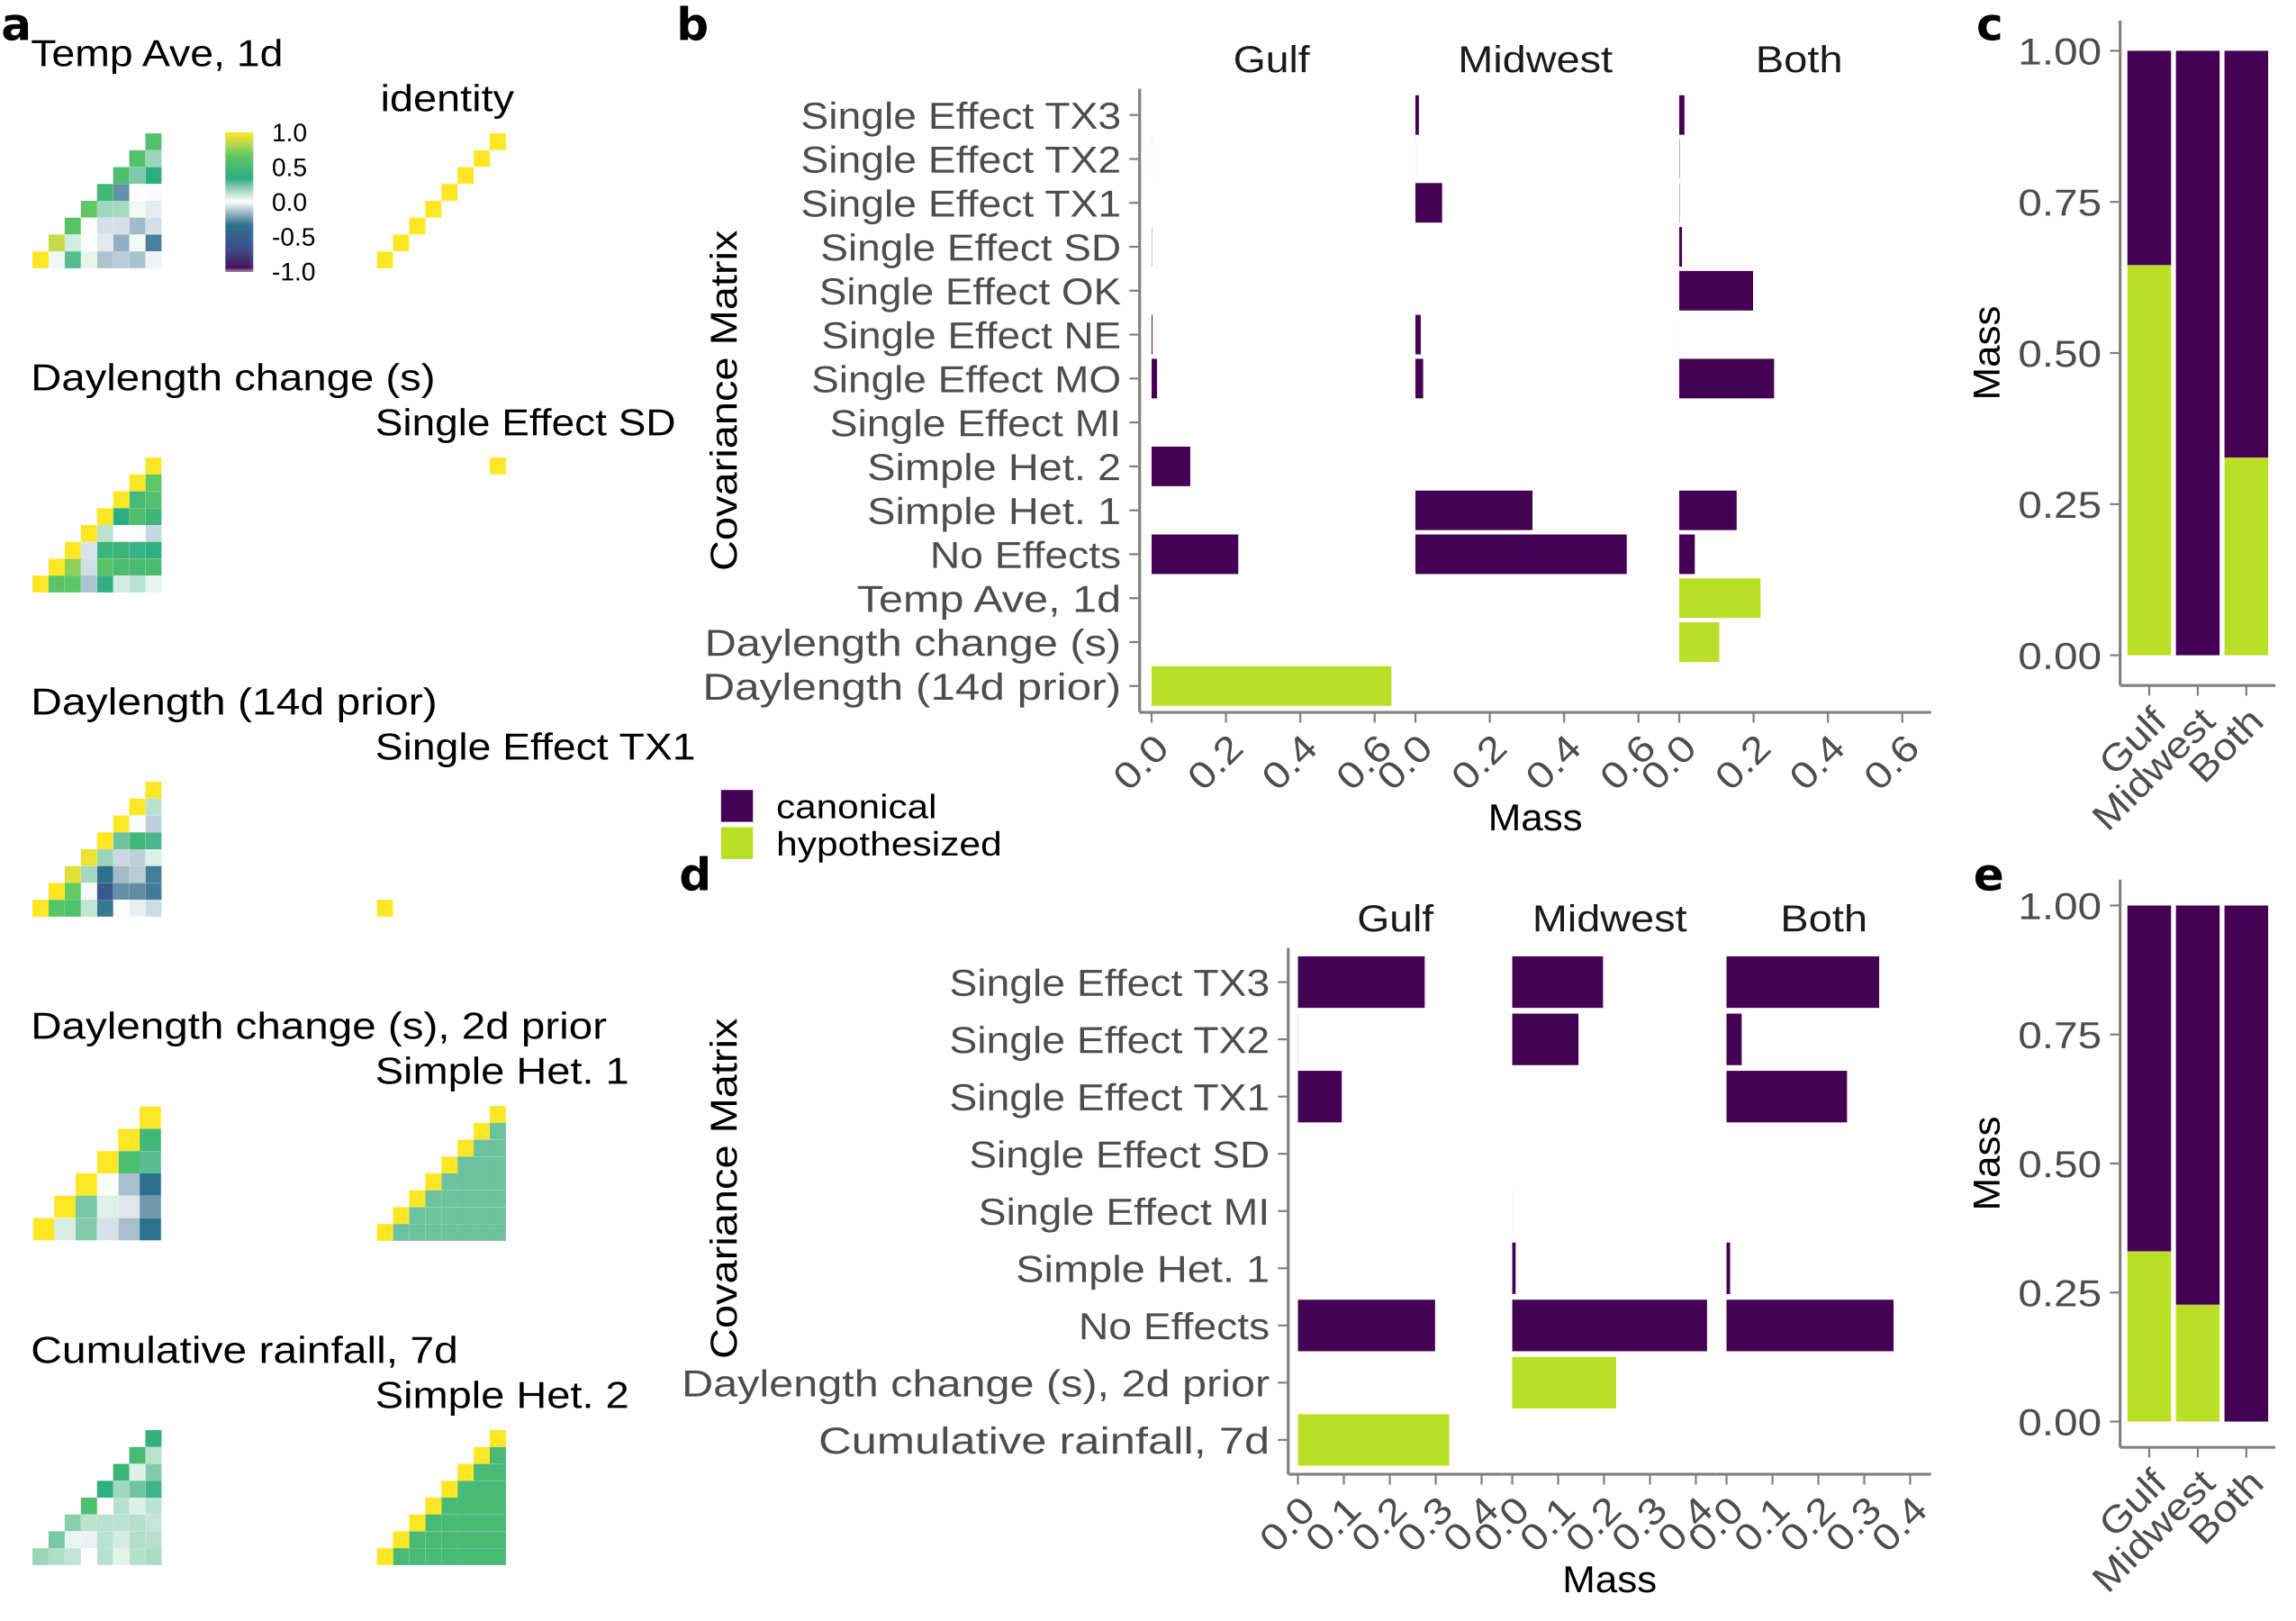
\includegraphics{images/Figure_2_Covariance_matrices_and_posterior_weights.png}

}

\caption{\label{fig-covar}Figure 2.}

\end{figure}%

\section{Materials and Methods}\label{materials-and-methods}

Whenever possible, plant material will be shared upon request. Source
data and code to replicate these analyses are available at:
https://github.com/Alice-MacQueen/pvdiv-phenology-gxe.git. SNP data to
replicate these analyses are available from the UT dataverse at
https://doi.org/link.

\subsubsection{Genotype-by-environment effects on green-up and flowering
as functions of weather-based
cues}\label{genotype-by-environment-effects-on-green-up-and-flowering-as-functions-of-weather-based-cues}

In 2019, we scored two phenological events every two days in two mapping
populations of switchgrass, a diversity panel and a pseudo-F2 cross,
planted at eight common garden locations (32, 34, 37). We scored
green-up date as the day of the year when 50\% of the tiller area of the
crown of the plant cut the previous year had green growth. Flowering
date was the day of the year when 50\% of the plant tillers had panicles
undergoing anthesis. We scored green-up and flowering as day of the
year, then linked these dates to multiple weather-based environmental
factors measured daily at each common garden (SI Appendix, Section S1,
Table S1).

The formation and resequencing of the diversity panel has been described
previously (32). The diversity panel contained 134 sequenced, clonally
propagated individuals from the Midwest genetic subpopulation, and 229
from the Gulf genetic subpopulation. To allow for the possibility that
different subpopulations had different strengths of connection between
our phenotypes and genotypes (38), we conducted three sets of genetic
analyses: on Gulf and Midwest genotypes separately, and on both
subpopulations together (`Both'). Analyses to determine narrow-sense
heritability (h2) for green-up and flowering were done using linear
mixed models and followed (32). Details on these models can be found in
(SI Appendix, Section S3,S4).

\subsubsection{Mapping major patterns of genotype-by-environment effects
on green-up and
flowering}\label{mapping-major-patterns-of-genotype-by-environment-effects-on-green-up-and-flowering-1}

To evaluate the prevalence and kinds of covariance patterns of SNP
effects across our common gardens, we used multivariate adaptive
shrinkage (mash) on SNP effect estimates from the diversity panel (35).
Mash is a statistical method that allows estimation and comparison of
many effects jointly across many different conditions; it improves on
previous methods by allowing multiple, arbitrary correlations in effect
sizes among conditions (SI Appendix, Section S5). To obtain SNP effect
estimates, we first conducted univariate genome-wide association at each
common garden for green-up and flowering date. We then analyzed SNP
effects for the top 19K relatively unlinked (r2 \textless{} 0.2) SNPs
per condition using mash, as in (32). Details on these models can be
found in (SI Appendix, Section S6).

We generated hypothesis-based covariance matrices derived from
correlations in environmental cues in the green-up or flowering date
windows for the three subpopulations (SI Appendix, Table S1, Section
S1). These covariance matrices represent correlations between identical
genotypes drawn from a specific population at pairs of common gardens;
covariances near one mean that the population has a strong, positive
linear relationship in individual responses at that pair of gardens,
while covariances near zero mean that there is no relationship within
the population for individual responses at that pair of gardens. Mash
SNP effects will undergo strong shrinkage towards one another in the
first case, and little shrinkage in the second case. Mash also generates
data-driven covariance matrices corresponding to major patterns of SNP
effects present in the data. We generated six data-driven matrices per
mash run, five (denoted DD\_PCA\_1 through DD\_PCA\_5) produced by
singular value decomposition (SVD) of an overall matrix, denoted
`DD\_tPCA'. We used SVD to present vectors of garden-specific effects
for each numbered DD\_PCA matrix, because the first eigenvector of a SVD
explains 100\% of the variation in these matrices, and each value in
this eigenvector represents one garden-specific effect.

Last, we characterized the overall patterns of antagonistic pleiotropy
in the set of SNPs where there was pairwise significance of effects at
pairs of gardens. To do this, we used the `get\_GxE' function of the
switchgrassGWAS R package. First, this determines the set of SNPs with
evidence of significant effects in both conditions for all pairs of
conditions using local false sign rates (lfsr) as the significance
criteria. Second, to determine antagonistic pleiotropy, this function
determines if effects significant in both conditions are of opposite
sign.

Using the lfsr rather than the local false discovery rate (lfdr) is a
critical change in our ability to detect antagonistic pleiotropy. The
lfdr, like other measures of FDR, focuses on if we have enough evidence
to reject the null hypothesis that an effect j is 0 -- that there is a
significant effect. Previous studies of antagonistic pleiotropy
(e.g.~(37)) have used the lfdr or equivalent statistical tests to detect
antagonistic pleiotropy. These tests were conservative, in that they
required two non-zero effects of different signs, while tests for
differential sensitivity required only one non-zero effect. This
previous work recognized that this testing bias could lead to
undercounting occurrences of antagonistic pleiotropy (26, 27), and
sought to reduce it by permutation (28). However, using the lfsr to test
for antagonistic pleiotropy does not undercount occurrences of
antagonistic pleiotropy, as this statistic answers a fundamentally
different question. For each effect j, the lfsr\_j is defined as the
probability that we make an error in the sign of effect j if we were
forced to declare the effect positive or negative (Stephens paper).
Thus, rather than asking ``Are these two effects different?'' - as we
reasonably expect two effects to be, even if this difference cannot be
measured - the local false sign rate answers a more meaningful question:
Can we be confident in the sign of this effect?

In addition, the get\_GxE function also sets an arbitrary threshold to
count an effect as changing in magnitude between environments, commonly
known as differential sensitivity. For differential sensitivity, this
function determines if effects significant in both conditions are of the
same sign and of a magnitude (not tested for significance) that differs
by a factor of 0.4 or more. The remaining effects that are significant
in both conditions have the same effect sign and similar effect
magnitudes and we denote these effects as having no GxE. The distinction
between effects with different magnitudes is arbitrary but useful to
fully characterize how effects vary across environments. and our use of
the lfsr to determine significance and our specification that SNP
effects must be significant in both conditions to be included means that
our tests for antagonistic pleiotropy carry an equal statistical burden
to those measuring differential sensitivity and effects without GxE.

\subsubsection{Confirmation of genotype-by-environment effects using an
independent mapping
population}\label{confirmation-of-genotype-by-environment-effects-using-an-independent-mapping-population-1}

To confirm candidate genomic regions and patterns of allelic effects
found in the diversity panel, we analyzed flowering in an outbred
pseudo-F2 cross between four individuals, two Midwest and two Gulf
individuals. The formation of this mapping population has been described
previously (34); additional details on QTL mapping can be found in SI
Appendix, Section S6. To be directly comparable to the diversity panel
data, only 2019 phenology data from the pseudo-F2 cross from the same
eight common garden sites were used. To compare our QTL enrichments of
significant mash associations to the null expectation, we used
permutation to choose 1000 sets of 23 genomic regions of the same size
randomly distributed throughout the genome, then calculated enrichments
of the mash 1\% tail in these random intervals.

\section{References}\label{references}

\bibsplit[2]

\phantomsection\label{refs}
\begin{CSLReferences}{0}{1}
\bibitem[\citeproctext]{ref-bauerle_photoperiodic_2012}
\CSLLeftMargin{1. }%
\CSLRightInline{W. L. Bauerle, \emph{et al.},
\href{https://doi.org/10.1073/pnas.1119131109}{Photoperiodic regulation
of the seasonal pattern of photosynthetic capacity and the implications
for carbon cycling}. \emph{Proceedings of the National Academy of
Sciences} \textbf{109}, 8612--8617 (2012).}

\bibitem[\citeproctext]{ref-andres2012genetic}
\CSLLeftMargin{2. }%
\CSLRightInline{F. Andrés, G. Coupland, The genetic basis of flowering
responses to seasonal cues. \emph{Nature Reviews Genetics} \textbf{13},
627--639 (2012).}

\bibitem[\citeproctext]{ref-korner2010phenology}
\CSLLeftMargin{3. }%
\CSLRightInline{C. Körner, D. Basler, Phenology under global warming.
\emph{Science} \textbf{327}, 1461--1462 (2010).}

\bibitem[\citeproctext]{ref-botero2015evolutionary}
\CSLLeftMargin{4. }%
\CSLRightInline{C. A. Botero, F. J. Weissing, J. Wright, D. R.
Rubenstein, Evolutionary tipping points in the capacity to adapt to
environmental change. \emph{Proceedings of the National Academy of
Sciences} \textbf{112}, 184--189 (2015).}

\bibitem[\citeproctext]{ref-blackman2013interacting}
\CSLLeftMargin{5. }%
\CSLRightInline{B. K. Blackman, Interacting duplications, fluctuating
selection, and convergence: The complex dynamics of flowering time
evolution during sunflower domestication. \emph{Journal of experimental
botany} \textbf{64}, 421--431 (2013).}

\bibitem[\citeproctext]{ref-henry2014transitions}
\CSLLeftMargin{6. }%
\CSLRightInline{L. P. Henry, R. H. Watson, B. K. Blackman, Transitions
in photoperiodic flowering are common and involve few loci in wild
sunflowers (helianthus; asteraceae). \emph{American Journal of Botany}
\textbf{101}, 1748--1758 (2014).}

\bibitem[\citeproctext]{ref-aagren2017adaptive}
\CSLLeftMargin{7. }%
\CSLRightInline{J. Ågren, C. G. Oakley, S. Lundemo, D. W. Schemske,
Adaptive divergence in flowering time among natural populations of
arabidopsis thaliana: Estimates of selection and QTL mapping.
\emph{Evolution} \textbf{71}, 550--564 (2017).}

\bibitem[\citeproctext]{ref-brachi2010linkage}
\CSLLeftMargin{8. }%
\CSLRightInline{B. Brachi, \emph{et al.}, Linkage and association
mapping of arabidopsis thaliana flowering time in nature. \emph{PLoS
genetics} \textbf{6}, e1000940 (2010).}

\bibitem[\citeproctext]{ref-dittmar2014flowering}
\CSLLeftMargin{9. }%
\CSLRightInline{E. L. Dittmar, C. G. Oakley, J. Ågren, D. W. Schemske,
Flowering time QTL in natural populations of arabidopsis thaliana and
implications for their adaptive value. \emph{Molecular ecology}
\textbf{23}, 4291--4303 (2014).}

\bibitem[\citeproctext]{ref-li2018genomic}
\CSLLeftMargin{10. }%
\CSLRightInline{X. Li, T. Guo, Q. Mu, X. Li, J. Yu, Genomic and
environmental determinants and their interplay underlying phenotypic
plasticity. \emph{Proceedings of the National Academy of Sciences}
\textbf{115}, 6679--6684 (2018).}

\bibitem[\citeproctext]{ref-romero2017study}
\CSLLeftMargin{11. }%
\CSLRightInline{J. A. Romero Navarro, \emph{et al.}, A study of allelic
diversity underlying flowering-time adaptation in maize landraces.
\emph{Nature genetics} \textbf{49}, 476--480 (2017).}

\bibitem[\citeproctext]{ref-wadgymar2017identifying}
\CSLLeftMargin{12. }%
\CSLRightInline{S. M. Wadgymar, \emph{et al.}, Identifying targets and
agents of selection: Innovative methods to evaluate the processes that
contribute to local adaptation. \emph{Methods in Ecology and Evolution}
\textbf{8}, 738--749 (2017).}

\bibitem[\citeproctext]{ref-blumel2015flowering}
\CSLLeftMargin{13. }%
\CSLRightInline{M. Blümel, N. Dally, C. Jung, Flowering time regulation
in crops---what did we learn from arabidopsis? \emph{Current opinion in
biotechnology} \textbf{32}, 121--129 (2015).}

\bibitem[\citeproctext]{ref-jung2009flowering}
\CSLLeftMargin{14. }%
\CSLRightInline{C. Jung, A. E. Müller, Flowering time control and
applications in plant breeding. \emph{Trends in plant science}
\textbf{14}, 563--573 (2009).}

\bibitem[\citeproctext]{ref-turner2005pseudo}
\CSLLeftMargin{15. }%
\CSLRightInline{A. Turner, J. Beales, S. Faure, R. P. Dunford, D. A.
Laurie, The pseudo-response regulator ppd-H1 provides adaptation to
photoperiod in barley. \emph{Science} \textbf{310}, 1031--1034 (2005).}

\bibitem[\citeproctext]{ref-faure2012mutation}
\CSLLeftMargin{16. }%
\CSLRightInline{S. Faure, \emph{et al.}, Mutation at the circadian clock
gene EARLY MATURITY 8 adapts domesticated barley (hordeum vulgare) to
short growing seasons. \emph{Proceedings of the National Academy of
Sciences} \textbf{109}, 8328--8333 (2012).}

\bibitem[\citeproctext]{ref-hung2012zmcct}
\CSLLeftMargin{17. }%
\CSLRightInline{H.-Y. Hung, \emph{et al.}, ZmCCT and the genetic basis
of day-length adaptation underlying the postdomestication spread of
maize. \emph{Proceedings of the National Academy of Sciences}
\textbf{109}, E1913--E1921 (2012).}

\bibitem[\citeproctext]{ref-zakhrabekova2012induced}
\CSLLeftMargin{18. }%
\CSLRightInline{S. Zakhrabekova, \emph{et al.}, Induced mutations in
circadian clock regulator mat-a facilitated short-season adaptation and
range extension in cultivated barley. \emph{Proceedings of the National
Academy of Sciences} \textbf{109}, 4326--4331 (2012).}

\bibitem[\citeproctext]{ref-yang2013oself3}
\CSLLeftMargin{19. }%
\CSLRightInline{Y. Yang, Q. Peng, G.-X. Chen, X.-H. Li, C.-Y. Wu, OsELF3
is involved in circadian clock regulation for promoting flowering under
long-day conditions in rice. \emph{Molecular Plant} \textbf{6}, 202--215
(2013).}

\bibitem[\citeproctext]{ref-pin2012multifaceted}
\CSLLeftMargin{20. }%
\CSLRightInline{P. Pin, O. Nilsson, The multifaceted roles of FLOWERING
LOCUS t in plant development. \emph{Plant, cell \& environment}
\textbf{35}, 1742--1755 (2012).}

\bibitem[\citeproctext]{ref-weller2019parallel}
\CSLLeftMargin{21. }%
\CSLRightInline{J. L. Weller, \emph{et al.}, Parallel origins of
photoperiod adaptation following dual domestications of common bean.
\emph{Journal of Experimental Botany} \textbf{70}, 1209--1219 (2019).}

\bibitem[\citeproctext]{ref-levene1953genetic}
\CSLLeftMargin{22. }%
\CSLRightInline{H. Levene, Genetic equilibrium when more than one
ecological niche is available. \emph{The American Naturalist}
\textbf{87}, 331--333 (1953).}

\bibitem[\citeproctext]{ref-felsenstein1976theoretical}
\CSLLeftMargin{23. }%
\CSLRightInline{J. Felsenstein, The theoretical population genetics of
variable selection and migration. \emph{Annual review of genetics}
\textbf{10}, 253--280 (1976).}

\bibitem[\citeproctext]{ref-kawecki2004conceptual}
\CSLLeftMargin{24. }%
\CSLRightInline{T. J. Kawecki, D. Ebert, Conceptual issues in local
adaptation. \emph{Ecology letters} \textbf{7}, 1225--1241 (2004).}

\bibitem[\citeproctext]{ref-hedrick1986genetic}
\CSLLeftMargin{25. }%
\CSLRightInline{P. W. Hedrick, Genetic polymorphism in heterogeneous
environments: A decade later. \emph{Annual review of ecology and
systematics} \textbf{17}, 535--566 (1986).}

\bibitem[\citeproctext]{ref-des2013genotype}
\CSLLeftMargin{26. }%
\CSLRightInline{D. L. Des Marais, K. M. Hernandez, T. E. Juenger,
Genotype-by-environment interaction and plasticity: Exploring genomic
responses of plants to the abiotic environment. \emph{Annual Review of
Ecology, Evolution, and Systematics} \textbf{44}, 5--29 (2013).}

\bibitem[\citeproctext]{ref-anderson2013genetic}
\CSLLeftMargin{27. }%
\CSLRightInline{J. T. Anderson, C.-R. Lee, C. A. Rushworth, R. I.
Colautti, T. Mitchell-Olds, Genetic trade-offs and conditional
neutrality contribute to local adaptation. \emph{Molecular ecology}
\textbf{22}, 699--708 (2013).}

\bibitem[\citeproctext]{ref-anderson2011evolutionary}
\CSLLeftMargin{28. }%
\CSLRightInline{J. T. Anderson, J. H. Willis, T. Mitchell-Olds,
Evolutionary genetics of plant adaptation. \emph{Trends in Genetics}
\textbf{27}, 258--266 (2011).}

\bibitem[\citeproctext]{ref-mitchell1997predicting}
\CSLLeftMargin{29. }%
\CSLRightInline{R. B. Mitchell, K. J. Moore, L. E. Moser, J. O. Fritz,
D. D. Redfearn, Predicting developmental morphology in switchgrass and
big bluestem. \emph{Agronomy Journal} \textbf{89}, 827--832 (1997).}

\bibitem[\citeproctext]{ref-parrish2005biology}
\CSLLeftMargin{30. }%
\CSLRightInline{D. J. Parrish, J. H. Fike, The biology and agronomy of
switchgrass for biofuels. \emph{BPTS} \textbf{24}, 423--459 (2005).}

\bibitem[\citeproctext]{ref-casler2004latitudinal}
\CSLLeftMargin{31. }%
\CSLRightInline{M. Casler, K. P. Vogel, C. Taliaferro, R. Wynia,
Latitudinal adaptation of switchgrass populations. \emph{Crop Science}
\textbf{44}, 293--303 (2004).}

\bibitem[\citeproctext]{ref-lovell2021genomic}
\CSLLeftMargin{32. }%
\CSLRightInline{J. T. Lovell, \emph{et al.}, Genomic mechanisms of
climate adaptation in polyploid bioenergy switchgrass. \emph{Nature}
\textbf{590}, 438--444 (2021).}

\bibitem[\citeproctext]{ref-porter1966analysis}
\CSLLeftMargin{33. }%
\CSLRightInline{C. L. Porter Jr, An analysis of variation between upland
and lowland switchgrass, panicum virgatum l., in central oklahoma.
\emph{Ecology} \textbf{47}, 980--992 (1966).}

\bibitem[\citeproctext]{ref-milano2016genetic}
\CSLLeftMargin{34. }%
\CSLRightInline{E. R. Milano, D. B. Lowry, T. E. Juenger, The genetic
basis of upland/lowland ecotype divergence in switchgrass (panicum
virgatum). \emph{G3: Genes, Genomes, Genetics} \textbf{6}, 3561--3570
(2016).}

\bibitem[\citeproctext]{ref-urbut2019flexible}
\CSLLeftMargin{35. }%
\CSLRightInline{S. M. Urbut, G. Wang, P. Carbonetto, M. Stephens,
Flexible statistical methods for estimating and testing effects in
genomic studies with multiple conditions. \emph{Nature genetics}
\textbf{51}, 187--195 (2019).}

\bibitem[\citeproctext]{ref-10.1093ux2fbiostatisticsux2fkxw041}
\CSLLeftMargin{36. }%
\CSLRightInline{M. Stephens,
\href{https://doi.org/10.1093/biostatistics/kxw041}{{False discovery
rates: a new deal}}. \emph{Biostatistics} \textbf{18}, 275--294 (2016).}

\end{CSLReferences}

\acknow{We thank the Brackenridge Field laboratory, the Ladybird Johnson
Wildflower Center, and the Juenger laboratory for support with plant
care and propagation. This material is based upon work supported in part
by the Great Lakes Bioenergy Research Center, U.S. Department of Energy,
Office of Science, Office of Biological and Environmental Research under
Award Numbers DE-SC0018409 and DE-FC02-07ER64494, the US Department of
Energy Awards DESC0014156 to T.E.J., DE-SC0017883 to D.B.L, National
Science Foundation PGRP Awards IOS0922457 and IOS1444533 to T.E.J, and
the Long-term Ecological Research Program (DEB 1832042) at the Kellogg
Biological Station.}

\showacknow{} % Display the acknowledgments section


\end{document}
